\documentclass[12pt]{article}
\usepackage[english]{babel}
\usepackage[utf8]{inputenc}
\usepackage[english]{babel}
\usepackage[a4paper, total={7.25in, 9.5in}]{geometry}
\usepackage{tikz-feynman}
\tikzfeynmanset{compat=1.0.0} 
\usepackage{subcaption}
\usepackage{float}
\floatplacement{figure}{H}
\usepackage{simpler-wick}
\usepackage{mathrsfs}  
\usepackage{dsfont}
\usepackage{relsize}
\usepackage{tikz-cd}
\DeclareMathAlphabet{\mathdutchcal}{U}{dutchcal}{m}{n}

\usepackage{cancel}



\newcommand{\field}{\hat{\Phi}}
\newcommand{\dfield}{\hat{\Phi}^\dagger}
 
\usepackage{amsthm, amssymb, amsmath, centernot}
\usepackage{slashed}
\newcommand{\notimplies}{%
  \mathrel{{\ooalign{\hidewidth$\not\phantom{=}$\hidewidth\cr$\implies$}}}}
 
\renewcommand\qedsymbol{$\square$}
\newcommand{\cont}{$\boxtimes$}
\newcommand{\divides}{\mid}
\newcommand{\ndivides}{\centernot \mid}

\newcommand{\Integers}{\mathbb{Z}}
\newcommand{\Natural}{\mathbb{N}}
\newcommand{\Complex}{\mathbb{C}}
\newcommand{\Zplus}{\mathbb{Z}^{+}}
\newcommand{\Primes}{\mathbb{P}}
\newcommand{\Q}{\mathbb{Q}}
\newcommand{\R}{\mathbb{R}}
\newcommand{\ball}[2]{B_{#1} \! \left(#2 \right)}
\newcommand{\Rplus}{\mathbb{R}^+}
\renewcommand{\Re}[1]{\mathrm{Re}\left[ #1 \right]}
\renewcommand{\Im}[1]{\mathrm{Im}\left[ #1 \right]}
\newcommand{\Op}{\mathcal{O}}

\newcommand{\invI}[2]{#1^{-1} \left( #2 \right)}
\newcommand{\End}[1]{\text{End}\left( A \right)}
\newcommand{\legsym}[2]{\left(\frac{#1}{#2} \right)}
\renewcommand{\mod}[3]{\: #1 \equiv #2 \: \mathrm{mod} \: #3 \:}
\newcommand{\nmod}[3]{\: #1 \centernot \equiv #2 \: mod \: #3 \:}
\newcommand{\ndiv}{\hspace{-4pt}\not \divides \hspace{2pt}}
\newcommand{\finfield}[1]{\mathbb{F}_{#1}}
\newcommand{\finunits}[1]{\mathbb{F}_{#1}^{\times}}
\newcommand{\ord}[1]{\mathrm{ord}\! \left(#1 \right)}
\newcommand{\quadfield}[1]{\Q \small(\sqrt{#1} \small)}
\newcommand{\vspan}[1]{\mathrm{span}\! \left\{#1 \right\}}
\newcommand{\galgroup}[1]{Gal \small(#1 \small)}
\newcommand{\bra}[1]{\left| #1 \right>}
\newcommand{\Oa}{O_\alpha}
\newcommand{\Od}{O_\alpha^{\dagger}}
\newcommand{\Oap}{O_{\alpha '}}
\newcommand{\Odp}{O_{\alpha '}^{\dagger}}
\newcommand{\im}[1]{\mathrm{im} \: #1}
\renewcommand{\ker}[1]{\mathrm{ker} \: #1}
\newcommand{\ket}[1]{\left| #1 \right>}
\renewcommand{\bra}[1]{\left< #1 \right|}
\newcommand{\inner}[2]{\left< #1 | #2 \right>}
\newcommand{\expect}[2]{\left< #1 \right| #2 \left| #1 \right>}
\renewcommand{\d}[1]{ \mathrm{d}#1 \:}
\newcommand{\dn}[2]{ \mathrm{d}^{#1} #2 \:}
\newcommand{\deriv}[2]{\frac{\d{#1}}{\d{#2}}}
\newcommand{\nderiv}[3]{\frac{\dn{#1}{#2}}{\d{#3^{#1}}}}
\newcommand{\pderiv}[2]{\frac{\partial{#1}}{\partial{#2}}}
\newcommand{\fderiv}[2]{\frac{\delta #1}{\delta #2}}
\newcommand{\parsq}[2]{\frac{\partial^2{#1}}{\partial{#2}^2}}
\newcommand{\topo}{\mathcal{T}}
\newcommand{\base}{\mathcal{B}}
\renewcommand{\bf}[1]{\mathbf{#1}}
\renewcommand{\a}{\hat{a}}
\newcommand{\adag}{\hat{a}^\dagger}
\renewcommand{\b}{\hat{b}}
\newcommand{\bdag}{\hat{b}^\dagger}
\renewcommand{\c}{\hat{c}}
\newcommand{\cdag}{\hat{c}^\dagger}
\newcommand{\hamilt}{\hat{H}}
\renewcommand{\L}{\hat{L}}
\newcommand{\Lz}{\hat{L}_z}
\newcommand{\Lsquared}{\hat{L}^2}
\renewcommand{\S}{\hat{S}}
\renewcommand{\empty}{\varnothing}
\newcommand{\J}{\hat{J}}
\newcommand{\lagrange}{\mathcal{L}}
\newcommand{\dfourx}{\mathrm{d}^4x}
\newcommand{\meson}{\phi}
\newcommand{\dpsi}{\psi^\dagger}
\newcommand{\ipic}{\mathrm{int}}
\newcommand{\tr}[1]{\mathrm{tr} \left( #1 \right)}
\newcommand{\C}{\mathbb{C}}
\newcommand{\CP}[1]{\mathbb{CP}^{#1}}
\newcommand{\Vol}[1]{\mathrm{Vol}\left(#1\right)}

\newcommand{\Tr}[1]{\mathrm{Tr}\left( #1 \right)}
\newcommand{\Charge}{\hat{\mathbf{C}}}
\newcommand{\Parity}{\hat{\mathbf{P}}}
\newcommand{\Time}{\hat{\mathbf{T}}}
\newcommand{\Torder}[1]{\mathbf{T}\left[ #1 \right]}
\newcommand{\Norder}[1]{\mathbf{N}\left[ #1 \right]}
\newcommand{\Znorm}{\mathcal{Z}}
\newcommand{\EV}[1]{\left< #1 \right>}
\newcommand{\interact}{\mathrm{int}}
\newcommand{\covD}{\mathcal{D}}
\newcommand{\conj}[1]{\overline{#1}}

\newcommand{\SO}[2]{\mathrm{SO}(#1, #2)}
\newcommand{\SU}[2]{\mathrm{SU}(#1, #2)}

\newcommand{\anticom}[2]{\left\{ #1 , #2 \right\}}


\newcommand{\pathd}[1]{\! \mathdutchcal{D} #1 \:}

\renewcommand{\theenumi}{(\alph{enumi})}


\renewcommand{\theenumi}{(\alph{enumi})}

\newcommand{\atitle}[1]{\title{% 
	\large \textbf{Physics GR8048 Quantum Field Theory II
	\\ Assignment \# #1} \vspace{-2ex}}
\author{Benjamin Church }
\maketitle}

\newcommand{\atitleIII}[1]{\title{% 
	\large \textbf{Physics GR8049 Quantum Field Theory III
	\\ Assignment \# #1} \vspace{-2ex}}
\author{Benjamin Church }
\maketitle}

\theoremstyle{definition}
\newtheorem{theorem}{Theorem}[section]
\newtheorem{definition}{definition}[section]
\newtheorem{lemma}[theorem]{Lemma}
\newtheorem{proposition}[theorem]{Proposition}
\newtheorem{corollary}[theorem]{Corollary}
\newtheorem{example}[theorem]{Example}
\newtheorem{remark}[theorem]{Remark}

\usepackage{slashed}
\begin{document}

\atitle{5}

\section*{Problem 1}
\subsection*{(a)}
In $D$ dimensions, the Lagrangian must have mass dimension $D$ such that the action is dimensionless. Using this fact,
consider the following theories in an arbitrary number of dimensions $D$. 

\subsection*{i.}
\[ \lagrange = \tfrac{1}{2} (\partial \phi)^2 - \tfrac{1}{2} m^2 \phi^2 - \tfrac{1}{4!} \lambda \phi^4 - \tfrac{1}{6!} \lambda' \phi^6 \]
The term $(\partial \phi)^2$ must have mass dimension $D$ so $\phi$ has mass dimension $\tfrac{1}{2} D - 1$. Therefore, the constant $m$ has dimension $1$ such that $2 \cdot (\tfrac{1}{2} D - 1) + 2 = D$. Furthermore, the constants $\lambda$ and $\lambda'$ have mass dimensions $D - 2 (D - 2) = 4 - D$ and $D - 3 (D - 2) = 6 - 2 D$ respectively. For the theory to be renormalizable, these dimensions must all be nonnegative. Thus, $4 - D \ge 0$ and $6 - 2 D \ge 0$ so $D \le 4$ and $D \le 3$. Therefore, for $D \le 3$ the theory is renormalizable and nonrenormalizable otherwise. For $D < 3$ strictly, all the coupling constants have positive mass dimension so the theory is super-renormalizable. 

\subsection*{ii.}

\[ \lagrange = \tfrac{1}{2} (1 + g \phi^2) (\partial \phi)^2 - \tfrac{1}{2} m^2 \phi^2 - \tfrac{1}{4!} \phi^4 \]
The term $(\partial \phi)^2$ must have mass dimension $D$ so $\phi$ has mass dimension $\tfrac{1}{2}D - 1$. Because $1$ and $g \phi^2$ must have the same mass dimension, we immediately see that $g$ must have mass dimension $1 - \tfrac{1}{2} D$. Furthermore, $[m] = 1$ and $[\lambda] = 4 - D$ as before. Therefore, for the theory to be renormalizable, these mass dimensions must all be nonnegative. Thus, $2 \ge D$ and $4 \ge D$. Therefore, the theory is super-renormalizable for $D < 2$, renormalizable for $D \le 2$, and nonrenormalizable otherwise. 

\subsection*{iii.}

\[ \lagrange = \bar{\psi} ( i \gamma^\mu  \partial_\mu - M) \psi - g (\bar{\psi} \psi)^2 \]
where $\psi$ is a spinor field. The term $\bar{\psi} i \slashed{\partial} \psi$ must have mass dimension $D$ and therefore $\phi$ has mass dimension $\tfrac{1}{2}(D - 1)$. Therefore, $[M] = 1$ and $[g] = D - 2 (D - 1) = 2 - D$. For these terms to have nonegative mass dimension, $D \le 2$. Therefore, the theory is super-renormalizable when $D < 2$, renormalizable when $D \le 2$, and nonrenormalizable otherwise. 

\subsection*{iv.}

\[ \lagrange = \tfrac{1}{2} (\partial \phi)^2 - \tfrac{1}{2} m^2 \phi^2 + \bar{\psi} ( i \gamma^\mu \partial_\mu - M) \psi - g \phi \bar{\psi} \psi \]
As before, $ [ \phi ] = \tfrac{1}{2} D - 1 $ and $[\psi] = \tfrac{1}{2}(D - 1)$. Therefore, $[m] = 1$ and $[M] = 1$. Finally, since $[g \phi \bar{\psi} \psi] = D$ we have $[g] = D - (\tfrac{1}{2} D - 1) - (D - 1) = 2 - \tfrac{1}{2} D$. Therefore, $D \le 4$ if we want $[g]$ to be nonnegative. Thus, when $D < 4$ the theory is super-renormalizable, when $D \le 4$ the theory is renormalizable, and the theory is nonrenormalizable otherwise. 

\subsection*{(b)}

In SI units, $[G] = \mathrm{kg}^{-1} \, \mathrm{m}^3 \, \mathrm{s}^{-2}$. Therefore, the mass dimension of $G$ is $-1 - 3 + 2 = -2$. Since the coupling constant has a negative mass dimension we should expect gravity to be non-renormalizable.  

\section*{Problem 2}

As discussed in the problem statement, to leading order in $N$ the one-particle irreducible diagrams are independent of incoming momenta because they only consist of loop systems which are attached to the propagator at one point and therefore the incoming momentum cannot flow through the loop. These diagrams produce a (UV divergent) shift to the mass which is independent of $p$ and therefore exactly canceled by the corresponding counterterm. Any loop system which is attached to a $\psi^a \psi^b \to \psi^a \psi^b$ scattering diagram at a single point is therefore exactly canceled by the a corresponding counterterm vertex inserted in the $\phi$ propagator. Thus, in the limit of large $N$ we need only consider diagrams consisting of linear bubble chains with any combination of regular and counterterm vertices. Since changing any vertex into a counterterm vertex gives annother valid diagram in the sum, we may simplify the calculation by incorporating these two types of vertices into a single vertex with coeficient $-i(g + c_g)$. Then, the sum over bubble chains gives an amplitude,
\[ i \mathcal{M} = \frac{-i(g + c_g)}{N} + N \left( \frac{-i(g + c_g)}{N} \right)^2 i V(t) + N^2 \left( \frac{-i(g + c_g)}{N} \right)^3 [i V(p)]^2 + \cdots \]
where $i V(p)$ is the amplitude of the single loop diagram with total incoming momentum $p$. This formula holds because there is always one more interaction vertex than the number of loops in the chain and the outgoing momentum of each loop is equal to its incoming momentum so each loop has a total of $p$ momentum flowing through it. We can simplify this amplitude by noting that the sum is a geometric series,

\[ i \mathcal{M} = \frac{-i(g + c_g)}{N} \left[ 1 + (g + c_g) V(p) + [(g + c_g) V(p)]^2 + \cdots \right] = \frac{-i(g + c_g)}{N} \cdot \frac{1}{1 - (g + c_g) V(p)} \]


\subsection*{Calculating the One-Loop Amplitude}

To find the total scattering cross section, we need to evaluate the integral over a single loop $V$. This integral is given by,
\[ i V(p) = \int \frac{\mathrm{d}^4 k}{(2\pi)^4} \frac{i}{k^2 - M^2 + i \epsilon} \cdot \frac{i}{(k + p)^2 - M^2 + i \epsilon} \]
This integral turns out to be exactly the same as the integral for the one-loop correction to the $\phi$ propagator in scalar Yukawa theory. Using dimensional regularization, I will reproduce the calculation here. We introduce Feynman parameters, Wick rotate, perform dimensional regularization, introduce a Schwinger parameter, and then integrate.

\begin{align*}
i V(p) & = \int \frac{\mathrm{d}^4 k}{(2\pi)^4} \frac{i}{k^2 - M^2 + i \epsilon} \cdot \frac{i}{(k + p)^2 - M^2 + i \epsilon} 
\\
& = - \int \frac{\mathrm{d}^4 k}{(2\pi)^4} \int \frac{ \d{x} \d{y} \delta(x + y - 1)}{[x k^2 + (k + p)^2 y - M^2 + i \epsilon]^2} 
\\
& = - \int \frac{\mathrm{d}^4 k}{(2\pi)^4} \int \frac{ \d{x} \d{y} \delta(x + y - 1)}{[k^2 + 2y  p \cdot k + y p^2 - M^2 + i \epsilon]^2} 
\\
& = - \int \frac{\mathrm{d}^4 k}{(2\pi)^4} \int \frac{ \d{x} \d{y} \delta(x + y - 1)}{[(k + yp)^2 - y^2 p^2 + y p^2 - M^2 + i \epsilon]^2} 
\\
& = -i \int \frac{\mathrm{d}^4 \ell_E}{(2\pi)^4} \int \frac{ \d{x} \d{y} \delta(x + y - 1)}{[\ell_E^2 + y^2 p^2 - y p^2 + M^2 - i \epsilon]^2} 
\end{align*}
Let $\Delta = y(y - 1) p^2 + M^2 - i \epsilon$. Now we integrate in $D = 4 - \delta$ dimensions,
\begin{align*}
i V(p) &= -i \int \frac{\mathrm{d}^D \ell_E}{(2\pi)^D} \int \frac{ \d{x} \d{y} \delta(x + y - 1)}{[\ell_E^2 + \Delta]^2} 
\\
& = -\frac{2i}{(4 \pi)^{\frac{D}{2}} \Gamma\left(\frac{D}{2}\right)} \int \frac{ \d{\ell_E} \: \ell_E^{D - 1} \: \d{x} \d{y} \delta(x + y - 1)}{[\ell_E^2 + \Delta]^2} 
\\
& = -\frac{2i}{(4 \pi)^{\frac{D}{2}} \Gamma\left(\frac{D}{2}\right)} \int \d{\ell_E} \: \ell_E^{D - 1} \: \d{x} \d{y} \delta(x + y - 1) \int \frac{\d{s}}{s} s^2 e^{-s(\ell_E^2 + \Delta)} 
\\
& = -\frac{2i}{(4 \pi)^{\frac{D}{2}} \Gamma\left(\frac{D}{2}\right)} \int \d{x} \d{y} \delta(x + y - 1) \int \frac{\d{s}}{s} s^2 e^{-s \Delta} \int \d{\ell_E} \: \ell_E^{D - 1} e^{-s \ell_E^2} 
\end{align*}
By a change of variables $u = s \ell_E$ we can write the integral,
\[ \int \d{\ell_E} \: \ell_E^{D - 1} e^{-s \ell_E^2}  = \frac{1}{2 s} \frac{1}{s^{\frac{D}{2} - 1}} \int \d{u} u^{\frac{D}{2} - 1} e^{-u} = \frac{\Gamma\left(\tfrac{D}{2}\right)}{2 s^{\frac{D}{2}}}  \]
Therefore,
\begin{align*}
i V(p) & = -\frac{i}{(4 \pi)^{\frac{D}{2}}} \int \d{x} \d{y} \delta(x + y - 1) \int \frac{\d{s}}{s} s^{2 - \tfrac{D}{2}} e^{-s \Delta} 
\\
& = -\frac{i}{(4 \pi)^{\frac{D}{2}}} \int \d{x} \d{y} \delta(x + y - 1) \: \Gamma\left(2 - \tfrac{D}{2}\right) \Delta^{2 - \tfrac{D}{2}}
\\
& = -\frac{i}{(4 \pi)^2} \int \d{x} \d{y} \delta(x + y - 1) \: \Gamma\left(2 - \tfrac{D}{2}\right) \left( \frac{\Delta}{4 \pi} \right)^{2 - \tfrac{D}{2}}
\\
& \xrightarrow{\delta \to 0} 
\frac{i}{(4 \pi)^2} \int \d{x} \d{y} \delta(x + y - 1) \: \left[ - \frac{2}{\delta} + \gamma_E  - \log{(4 \pi)} + \log{\Delta} \right]
\\
& = \frac{i}{16 \pi^2} \left[ - \frac{2}{\delta} + \gamma_E - \log{(4 \pi)} + \int_0^1 \d{x} \log{[x(x-1) p^2 + M^2 - i \epsilon]} \right]
\end{align*}
The total momentum flowing into the bubble chain is $p = p_1 - p_1'$ we have $p^2 = (p_1 - p_1')^2 = t$ so we can write the one-loop amplitude as a function of the Mandelstam variable $t$,
\[ V(t) = \frac{1}{16 \pi^2} \left[ - \frac{2}{\delta} + \gamma_E - \log{(4 \pi)} + \int_0^1 \d{x} \log{[x(x-1) t + M^2 - i \epsilon]} \right] \]
Last time, we analytically computed the behavior of this integral. I will not reproduce the argument, only quote the result,

\[ \int_0^1 \d{x} \log{[x(x-1) t + M^2 - i \epsilon]} = -2 + 2 \left( \sqrt{\frac{4 M^2 - t}{-t}} \right) \mathrm{arctanh} \left( \sqrt{\frac{-t}{4 M^2 - t}} \right) + 2 \log{M} \]

for $ t < 0$ which luckily is the only case we care about for two-particle scattering.

\subsection*{Renormalization} 

The scattering amplitude for $\psi^a \psi^b \to \psi^a \psi^b$ is given by,
\[ i \mathcal{M} = \frac{1}{N} \cdot \frac{-i (g + c_g)}{1 - (g + c_g) V(t)} \]
However, the integral $V(p)$ is horribly divergent. Therefore, we must set the counterterm $c_g$ to cancel this divergence. We will take the renormalization condition $i \mathcal{M} = - i \frac{g}{N}$ at zero momentum, that is, $s = (2 M)^2$ and $t = u = 0$. Define,
\[Q =  V(t = 0) = \frac{1}{16 \pi^2} \left[ - \frac{2}{\delta} + \gamma_E - \log{(4 \pi)} + \int_0^1 \d{x} \log{[M^2 - i \epsilon]} \right]  = \frac{1}{16 \pi^2} \left[ - \frac{2}{\delta} + \gamma_E - \log{(4 \pi)} + 2 \log{M} \right]  \]
where I have taken the limit $\epsilon \to 0$ since the integral has no branch cuts since $M > 0$. 
Then the renormalization condition fixes,
\begin{align*}
\frac{1}{N} \cdot \frac{-i (g + c_g)}{1 - (g + c_g) Q} = - \frac{ig}{N}
\end{align*} 
And therefore,
\[ g + c_g = g(1 - (g + c_g) Q)\] 
which sets,
\[ c_g = -\frac{g^2 Q}{1 + g Q}\]
Given this value for the counterterm, the quantity,
\[ g + c_g = g - g^2 \frac{Q}{1+gQ} = \frac{g + g^2 Q - g^2 Q}{1 + g Q} = \frac{g}{1 + g Q} \]
will be very usefull. Using these relations, the scattering amplitude becomes,
\[ i\mathcal{M} = - \frac{i}{N} \cdot \frac{g}{1 + g Q} \frac{1}{1 - \frac{g}{1 + g Q} V(t)} = - \frac{ig}{N} \cdot  \frac{1}{1 + g Q - g V(t)} = \frac{-ig}{N} \cdot \frac{1}{1 - g (V(t) - Q)} \]
Therefore, we should consider the term,
\[ V(t) - Q = \frac{1}{16 \pi^2} \int_0^1 \d{x} \log{\left[ \frac{x(1-x)|t| + M^2}{M^2} \right]} = \frac{1}{16 \pi^2} \left[ -2 + 2 \left( \sqrt{\frac{4 M^2 + |t|}{|t|}} \right) \mathrm{arctanh} \left( \sqrt{\frac{|t|}{4 M^2 + |t|}} \right) \right] \]
where we can drop the $i \epsilon$ because the argument of the log is positive and nowhere near the branch cut. Therefore,
\[ i \mathcal{M} = \frac{-ig}{N} \cdot \frac{1}{1 - \frac{g}{16 \pi^2} \int_0^1 \d{x} \log{\left[ \frac{x(1-x) |t| + M^2}{M^2} \right]}}  = \frac{-ig}{N} \cdot \frac{1}{1 - \frac{g}{16 \pi^2} \left[ -2 + 2 \left( \sqrt{\frac{4 M^2 + |t|}{|t|}} \right) \mathrm{arctanh} \left( \sqrt{\frac{|t|}{4 M^2 + |t|}} \right) \right]} \]

\subsection*{High Energy Behavior}

\begin{figure}
\begin{center}
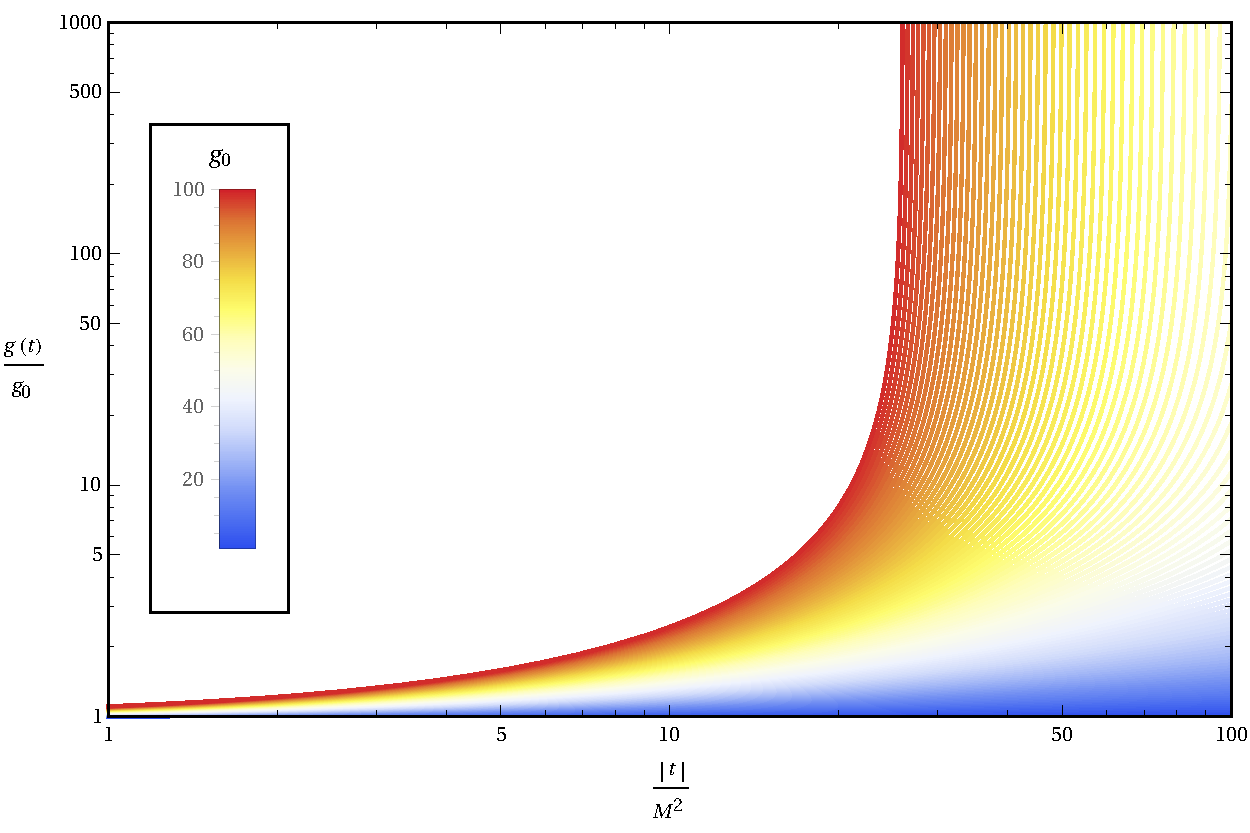
\includegraphics[width = 12cm, height = 8cm]{CouplingConstant}
\caption{Effective coupling constant as a function of energy scale and zero energy coupling strength $g_0$. Scale is log-log. Note the pole in $g(t)$ and its dependence on $g_0$. }
\label{scattering}
\end{center}
\end{figure}

In figure \ref{scattering}. there is a high energy pole at which the effective coupling constant and thus scattering amplitude becomes infinite. The position of this pole depends on the renormalized coupling constant of the theory $g = g_0$ fixed at zero energy. To find the value of $E_*$ at which the theory becomes infinitely strongly coupled we must solve the equation,
\[\frac{8 \pi^2}{g} + 1 = \left( \sqrt{\frac{4 M^2 + |t|}{|t|}} \right) \mathrm{arctanh} \left( \sqrt{\frac{|t|}{4 M^2 + |t|}} \right) \]
which is unfortunately rather transcendental. We can plot the numerical solutions to this equation as a funtion of $g$ but not find an exact form. However, under the assumption that $|t_*| \gg M^2$ which is equivalent to the assumption that $g$ is small we can solve this condition exactly. Using the integral expression directly, 
\begin{align*}
\int_0^1 \d{x} \log{\left[ \frac{x(1-x)|t| + M^2}{M^2} \right]} & = \int_0^1 \d{x} \log{\left[ x(1 - x) \frac{|t|}{M^2} + 1 \right]} \approx \int_0^1 \d{x} \log{\left[ x(1 - x) \frac{|t|}{M^2} \right]}
\\
& = \int_0^1 \left[ \log{x} + \log{(1-x)} \right] + \log{\frac{|t|}{M^2}}  = -2 + \log{\frac{|t|}{M^2}}
\end{align*}
Therefore, suppose that,
\[ 1 = \frac{g}{16 \pi^2} \left[-2 + \log{\frac{|t|}{M^2}} \right] \]
then we have,
\[ |t_*| = M^2 \exp{\left[16 \pi^2 g^{-1} + 2\right]} \]
However, we can write $t = (p_1 - p_1')^2 = -2 \vec{p}^{\, 2}(1 - \cos{\Theta})$ so at a fixed energy the maximum value for $|t|$ is $-4 \vec{p}^{\, 2} = - 4 (E^2 - M^2)$. Therefore, the minimum value for which infinite coupling appears (for backscattering) is,
\[ E_*^2 = |t_*|/4 + M^2 = M^2( \tfrac{1}{4} \exp{\left[16\pi^2 g^{-1} + 2\right]}  + 1) \]

\begin{figure}
\begin{center}
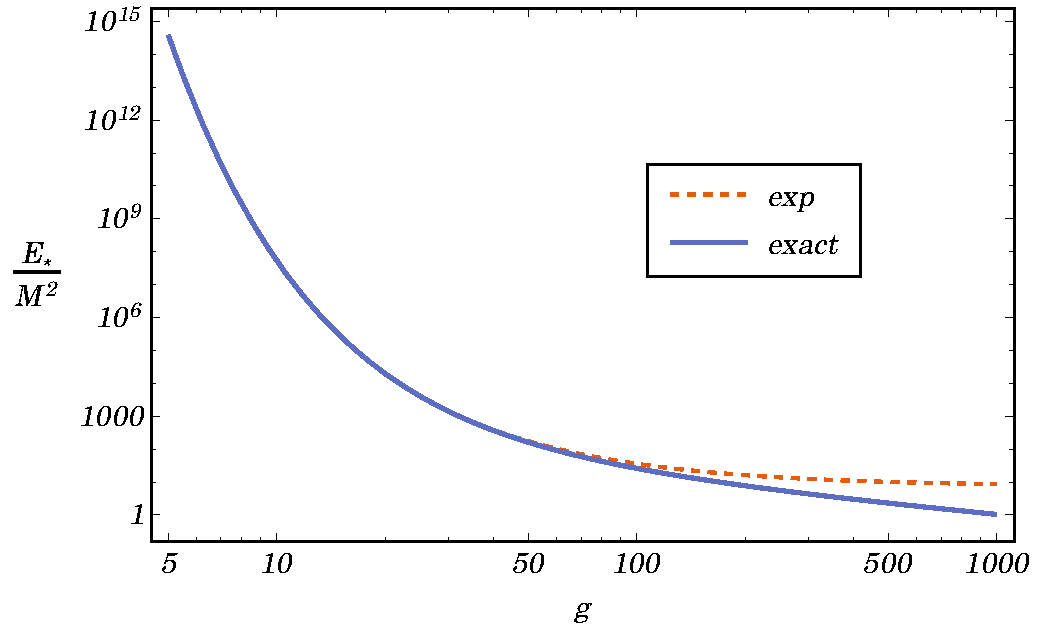
\includegraphics[width = 10cm, height = 6cm]{PoleEnergy}
\caption{Energy at which the theory becomes infinitely coupled as a function of the renormalized (at zero energy) coupling constant $g$. The scale is log-log.}
\label{pole}
\end{center}
\end{figure}

\section*{Problem 3}

\subsection*{(a)}

We will now illustrate a different renormlaization condition. We will define the variables, 
\[\bar{g} = - N \mathcal{M}(t = 0) = \frac{g + c_g}{1 - (g + c_g) Q} \]
and the scale-dependent coupling constant,
\[ g(\mu) = - N \mathcal{M}(t = -\mu^2) = \frac{g + c_g}{1 - (g + c_g) V(-\mu^2)} \]
If we choose to renormalize at the point $ g = g(\mu)$ for some fixed value of $\mu$ then, as before,
\[ c_g = -\frac{g^2 V(-\mu^2)}{1 + g V(-\mu^2)} \]
and thus,
\[ g + c_g = \frac{g}{1 + g V(-\mu^2)} \]
so plugging in,
\[ i\mathcal{M} = - \frac{ig(\mu)}{N} \cdot  \frac{1}{1 + g(\mu) V(-\mu^2) - g(\mu) V(t)} = - \frac{ig(\mu)}{N} \cdot \frac{1}{1 - g(\mu) [ V(t) - V(-\mu^2)]} \]
Furthermore, we can find the value of $g(\mu)$ directly from our earlier expressions in terms of $\bar{g}$. Using either of the above expressions,
\[ \frac{-i g(\mu)}{N} = i \mathcal{M}(-\mu^2) = - \frac{i g(0)}{N} \cdot \frac{1}{1 - g(0) [ V(-\mu^2) - V(0)]} = - \frac{i \bar{g}}{N} \cdot \frac{1}{1 - \bar{g} [ V(-\mu^2) - Q]} \]
Therefore,
\[ g(\mu) = \frac{\bar{g}}{1 - \bar{g} [V(-\mu^2) - Q]} = \frac{\bar{g}}{1 - \frac{\bar{g}}{16 \pi^2} \left[ -2 + 2 \left( \sqrt{\frac{4 M^2 + \mu^2}{\mu^2}} \right) \mathrm{arctanh} \left( \sqrt{\frac{\mu^2}{4 M^2 + \mu^2}} \right) \right] } \]
We can calculate this quantitiy in the limit $\mu^2 \gg M^2$ directly from the integral expression,
\[\int_0^1 \d{x} \log{\left[ \frac{x(1-x)\mu^2 + M^2}{M^2} \right]} \approx \int_0^1 \d{x} \log{\left[ x(1 - x) \frac{\mu^2}{M^2} \right]} = -2 + \log{\frac{\mu^2}{M^2}}\]
Therefore,
\[ g(\mu) = \frac{16 \pi^2 \bar{g}}{16 \pi^2 + 2 \bar{g} - \bar{g} \log{\frac{\mu^2}{M^2}}} \]
Now, we can solve for $\bar{g}$ to rexpress the scattering amplitude in terms of $g(\mu)$. 
We have,
\[ g(\mu) (1 - \bar{g} [V(-\mu^2) - Q]) = \bar{g} \]
and thus,
\[ \bar{g} = \frac{g(\mu)}{1 + g(\mu) [ V(-\mu^2) - Q]}\]
Writing the scattering amplitude in terms of $\bar{g}$ as before,
\begin{align*}
i \mathcal{M}(t) &= -\frac{i\bar{g}}{N} \cdot \frac{1}{1 - \bar{g} [V(t) - Q]} = -\frac{ig(\mu)}{N} \cdot \frac{1}{1 + g(\mu) [ V(-\mu^2) - Q]} \cdot \frac{1}{1 - g(\mu) \frac{V(t) - Q}{1 + g(\mu) [ V(-\mu^2) - Q] }}
\\
& = - \frac{i g(\mu)}{N} \cdot \frac{1}{1 - g(\mu)[V(t) - V(-\mu^2)]}
\end{align*}
which is the same expression we calculated earlier. \bigskip\\
Now, consider the integral quantity in this expression for the scattering amplitude,
\[ V(t) - V(-\mu^2) = \frac{1}{16 \pi^2} \int_0^1 \d{x} \log{\left[\frac{x(1-x)|t| + M^2}{x(1-x) \mu^2 + M^2}\right]}\]
In the limit $\mu^2 \gg M^2$ and $|t| \gg M^2$, we can see the limiting value of $V(t) - V(-\mu^2)$ directly from the integral,
\begin{align*}
V(t) - V(-\mu^2) &= \frac{1}{16 \pi^2} \int_0^1 \d{x} \log{\left[\frac{x(1-x)|t|/M^2 + 1}{x(1-x) \mu^2/M^2 + 1}\right]} \approx \frac{1}{16 \pi^2} \int_0^1 \d{x} \log{\left[\frac{x(1-x)|t|}{x(1-x) \mu^2}\right]}
\\
& = \frac{1}{16 \pi^2} \int_0^1 \d{x} \log{\frac{|t|}{\mu^2}} = \frac{1}{16 \pi^2} \log{\frac{|t|}{\mu^2}} 
\end{align*}
Therefore, the scattering amplitude becomes,
\[ i\mathcal{M} = - \frac{i g(\mu)}{N} \cdot \frac{1}{1 - \frac{g(\mu)}{16 \pi^2} \log{\frac{|t|}{\mu^2}}} \]
Unlike the expression in terms of $\bar{g}$, here, the mass does not appear explicilty so this expression is well-defined and non-singular in the limit $M \to 0$. Furthermore. in the limit $t \to 0$ we have, $-\log{\frac{|t|}{\mu^2}} \to \infty$ and thus, $i \mathcal{M} \to 0$. Therefore, the massless particles become decoupled at low energy.

\subsection*{(b)}
We can derive this result directly from the Feynman diagram expansion. We choose the renormalization condition $g = g(\mu)$. Then, consider the amplitude, 
\[g(e^\varepsilon \mu) = -N \mathcal{M}(t = -(e^\varepsilon \mu)^2) \]
Consider the Feynman diagram expansion to leading order in $\frac{1}{N}$, 
which give ampltudes,
\[ i\mathcal{M} = -\frac{ig}{N} + -\frac{ic_g}{N} + N \left(\frac{-ig}{N}\right)^2 iV(t) + \cdots \] 
Using our renormalization condition,
\[ -\frac{ig}{N} = -\frac{ig}{N} + -\frac{ic_g}{N} + \frac{-i g^2}{N} V(-\mu^2) + \cdots \]
and therefore,
\[ i\mathcal{M} = -\frac{ig}{N} - \frac{i g^2}{N} [V(t) - V(-\mu^2)] + \cdots \] 
In particular,
\[ g(e^\varepsilon \mu) = - N \mathcal{M}(t = - (e^\epsilon \mu)^2) = g + g^2 [V(-(e^\varepsilon \mu)^2) - V(-\mu^2)] + \cdots \] 
where the higher terms depend on larger powers in $V(-(e^\varepsilon \mu)^2) - V(-\mu^2)$. 
Now, in the limit $\mu^2 \gg M^2$, consider,
\begin{align*}
V(-(e^\varepsilon \mu)^2) - V(-\mu^2) & = \frac{1}{16\pi^2} \int_0^1 \d{x} \log{\left[ \frac{x(1-x) e^{2\varepsilon} \mu^2 + M^2}{x(1-x)\mu^2 + M^2} \right]} = \frac{1}{16\pi^2} \int_0^1 \d{x} \log{\left[ \frac{x(1-x) e^{2\varepsilon} \mu^2/M^2 + 1}{x(1-x)\mu^2/M^2 + 1} \right]} 
\\
& \approx
\frac{1}{16\pi^2} \int_0^1 \d{x} \log{\left[ \frac{x(1-x) e^{2\varepsilon} \mu^2}{x(1-x)\mu^2} \right]} = \frac{1}{16 \pi^2} \int_0^1 \d{x} \log{e^{2 \epsilon}} = \frac{\epsilon}{8 \pi^2} 
\end{align*}
Therefore, because $V(-(e^\varepsilon \mu)^2) - V(-\mu^2)$ is order $\epsilon$ and the latter terms contain higher powers of this quantity,
\[ g(e^\varepsilon \mu) = g + g^2 \frac{\epsilon}{8 \pi^2} + O(\epsilon^2) \] 
Using this result, and employing the renormalization condition $g = g(\mu)$, we can write,
\[ g(e^\varepsilon \mu) = g(\mu) + \frac{g(\mu)^2}{8 \pi^2} \epsilon + O(\epsilon^2) \] 
Therefore,
\[ \deriv{g}{\log{\mu}} = \frac{g(\mu)^2}{8 \pi^2} = \beta(g(\mu)) \quad \text{where} \quad \beta(g) = \frac{g^2}{8 \pi^2} \]
Integrating this differential equation,
\[ \int_{g_0}^{g(\mu)} \frac{\d{g}}{g^2} = \int_{\log{\mu_0}}^{\log{\mu}} \frac{\d{\log{\mu}}}{8 \pi^2} \implies \frac{1}{g_0} - \frac{1}{g(\mu)} = \frac{1}{8 \pi^2} \log{\frac{\mu}{\mu_0}} \]
which becomes,
\[ g(\mu) = \frac{g_0}{1 - \frac{g_0}{8\pi^2} \log{\frac{\mu}{\mu_0}}} \]
Since by definition $i \mathcal{M}(t = - \mu^2) = -\frac{ig(\mu)}{N}$ we have also found the scattering amplitude at any energy scale. Setting, $\mu = \sqrt{|t|}$ we get,
\[ i \mathcal{M} = - \frac{ig_0}{N} \cdot \frac{1}{1 - \frac{g_0}{8 \pi^2} \log{\frac{\sqrt{|t|}}{\mu_0}}} = - \frac{ig(\mu_0)}{N} \cdot \frac{1}{1 - \frac{g(\mu_0)}{16 \pi^2} \log{\frac{|t|}{\mu_0^2}}} \]
This is an identical expression for the scattering amplitude derived in the previous section renormalized at the point $\mu_0$.
\end{document}